\begin{figure}[ht]
\begin{center}
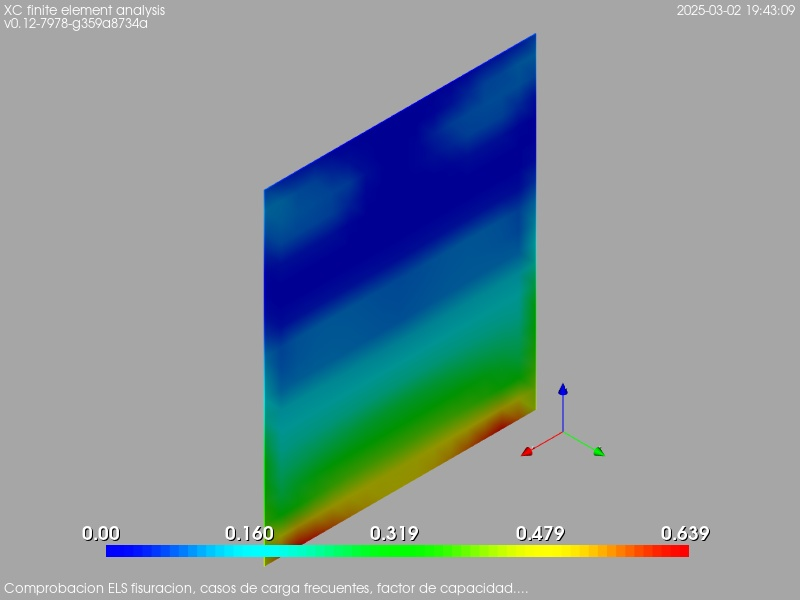
\includegraphics[width=\linewidth]{results/graphics/crackingSLS_freq/wallCFSect1}
\caption{Comprobación ELS fisuración, casos de carga frecuentes. Wall, factor de capacidad, dir. 1}
\label{SLS_frequentLoadsCrackControlwallCFSect1}
\end{center}
\end{figure}
\begin{figure}[ht]
\begin{center}
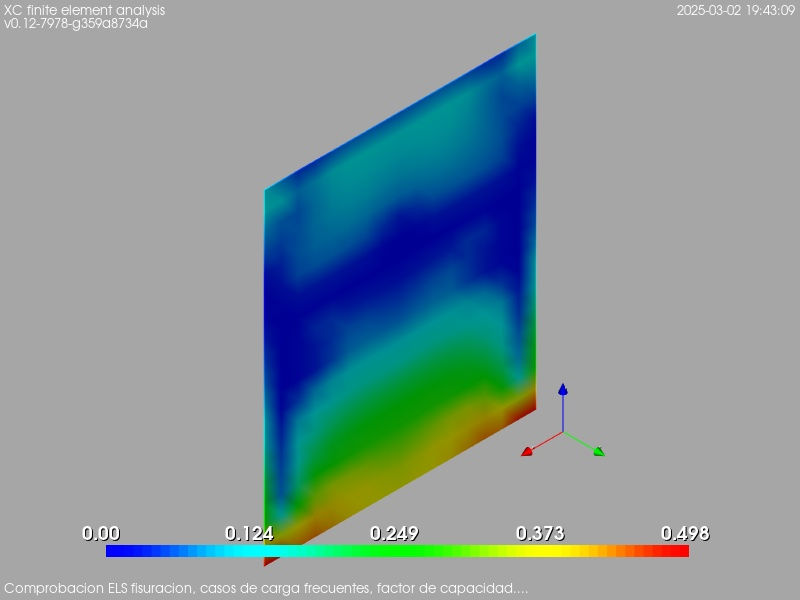
\includegraphics[width=\linewidth]{results/graphics/crackingSLS_freq/wallCFSect2}
\caption{Comprobación ELS fisuración, casos de carga frecuentes. Wall, factor de capacidad, dir. 2}
\label{SLS_frequentLoadsCrackControlwallCFSect2}
\end{center}
\end{figure}
\begin{figure}[ht]
\begin{center}
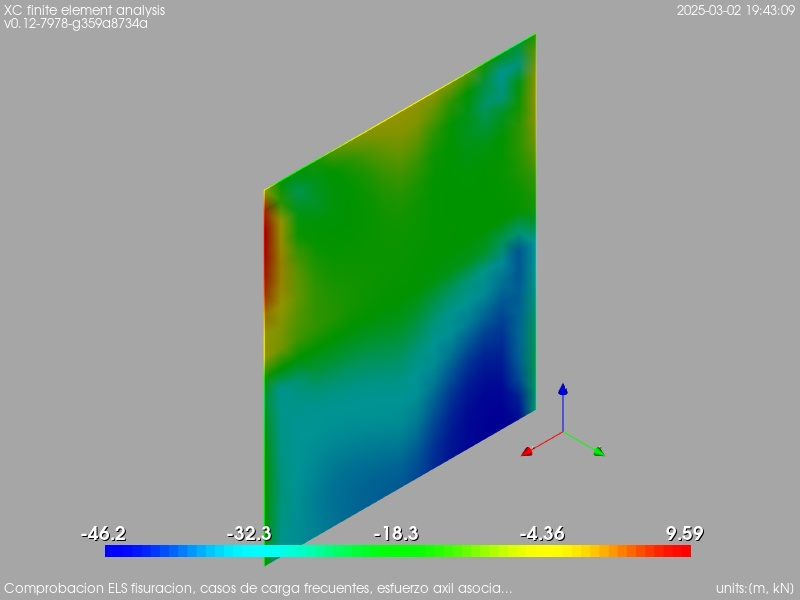
\includegraphics[width=\linewidth]{results/graphics/crackingSLS_freq/wallNSect1}
\caption{Comprobación ELS fisuración, casos de carga frecuentes. Wall, esfuerzo axil asociado al factor de capacidad, dir. 1}
\label{SLS_frequentLoadsCrackControlwallNSect1}
\end{center}
\end{figure}
\begin{figure}[ht]
\begin{center}
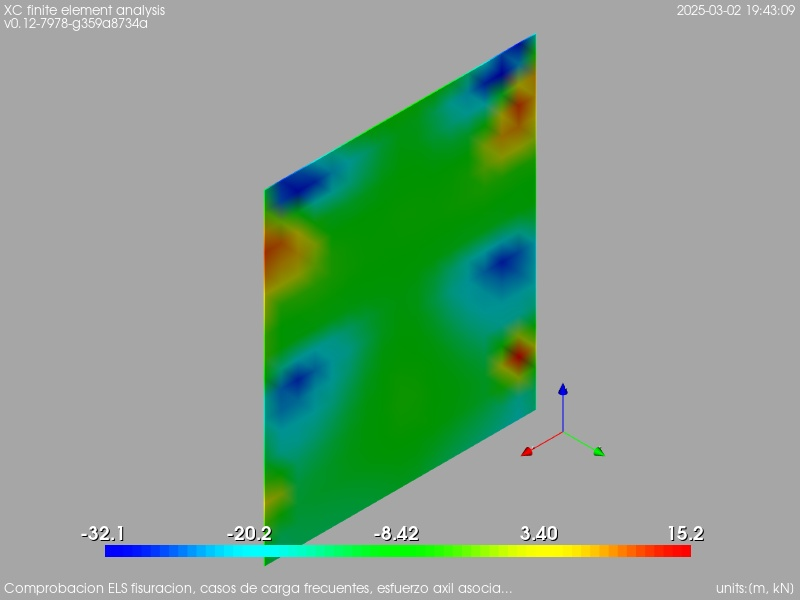
\includegraphics[width=\linewidth]{results/graphics/crackingSLS_freq/wallNSect2}
\caption{Comprobación ELS fisuración, casos de carga frecuentes. Wall, esfuerzo axil asociado al factor de capacidad, dir. 2}
\label{SLS_frequentLoadsCrackControlwallNSect2}
\end{center}
\end{figure}
\begin{figure}[ht]
\begin{center}
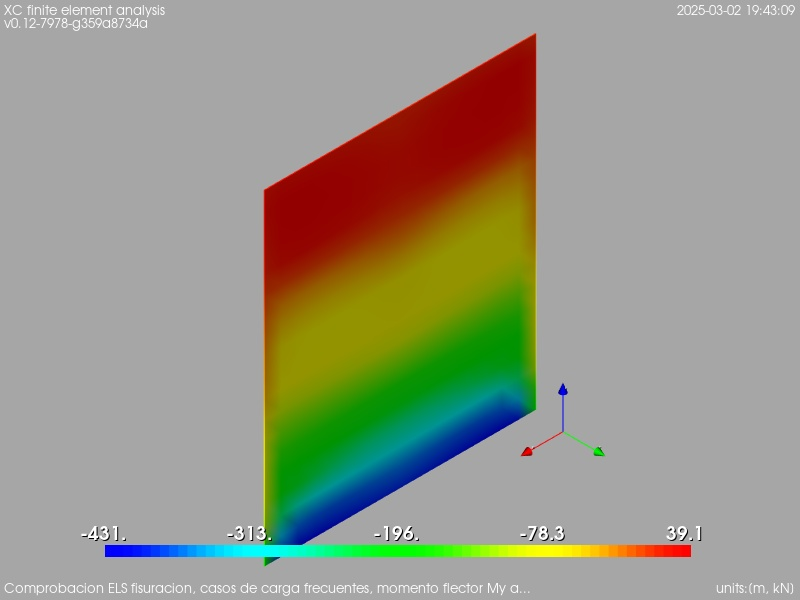
\includegraphics[width=\linewidth]{results/graphics/crackingSLS_freq/wallMySect1}
\caption{Comprobación ELS fisuración, casos de carga frecuentes. Wall, momento flector My asociado al factor de capacidad, dir. 1}
\label{SLS_frequentLoadsCrackControlwallMySect1}
\end{center}
\end{figure}
\begin{figure}[ht]
\begin{center}
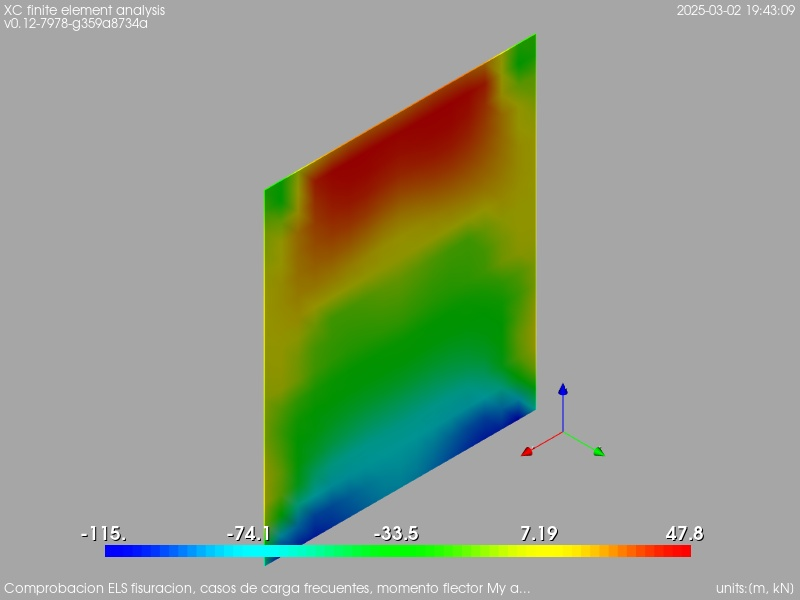
\includegraphics[width=\linewidth]{results/graphics/crackingSLS_freq/wallMySect2}
\caption{Comprobación ELS fisuración, casos de carga frecuentes. Wall, momento flector My asociado al factor de capacidad, dir. 2}
\label{SLS_frequentLoadsCrackControlwallMySect2}
\end{center}
\end{figure}
\begin{figure}[ht]
\begin{center}
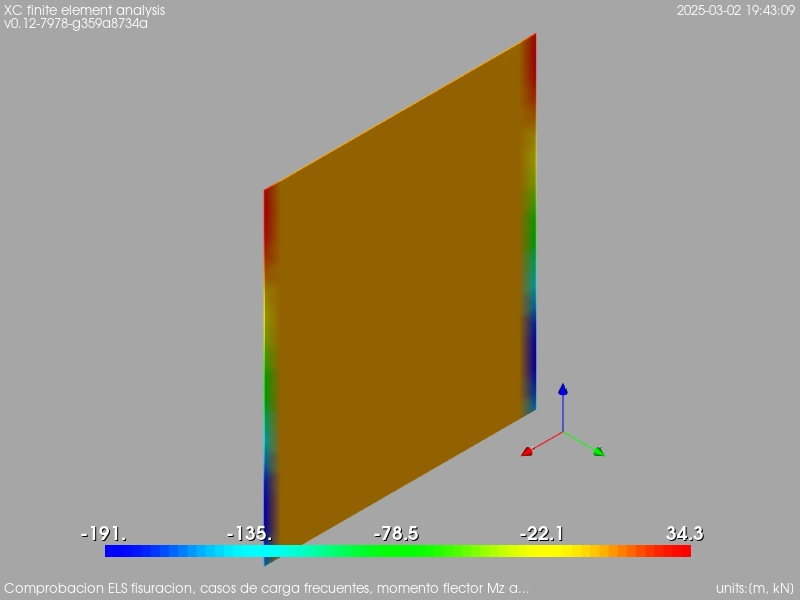
\includegraphics[width=\linewidth]{results/graphics/crackingSLS_freq/wallMzSect1}
\caption{Comprobación ELS fisuración, casos de carga frecuentes. Wall, momento flector Mz asociado al factor de capacidad, dir. 1}
\label{SLS_frequentLoadsCrackControlwallMzSect1}
\end{center}
\end{figure}
\begin{figure}[ht]
\begin{center}
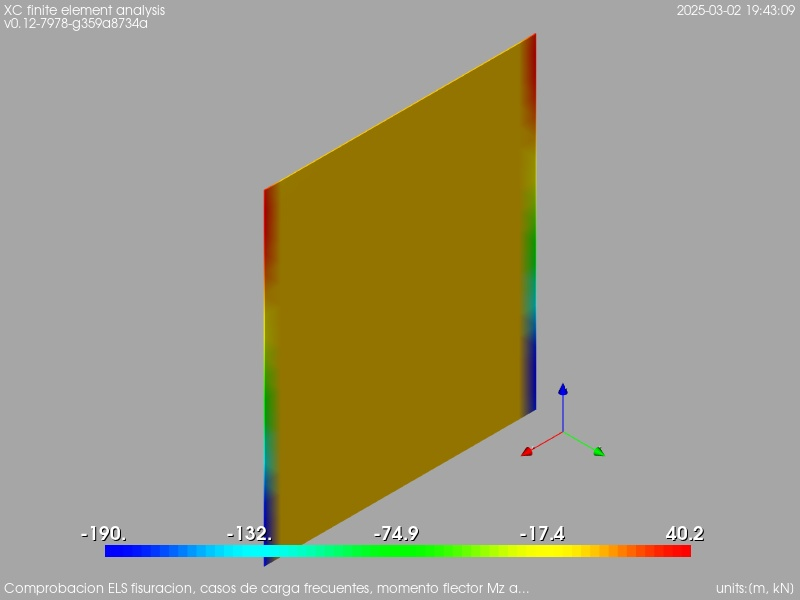
\includegraphics[width=\linewidth]{results/graphics/crackingSLS_freq/wallMzSect2}
\caption{Comprobación ELS fisuración, casos de carga frecuentes. Wall, momento flector Mz asociado al factor de capacidad, dir. 2}
\label{SLS_frequentLoadsCrackControlwallMzSect2}
\end{center}
\end{figure}
\begin{figure}[ht]
\begin{center}
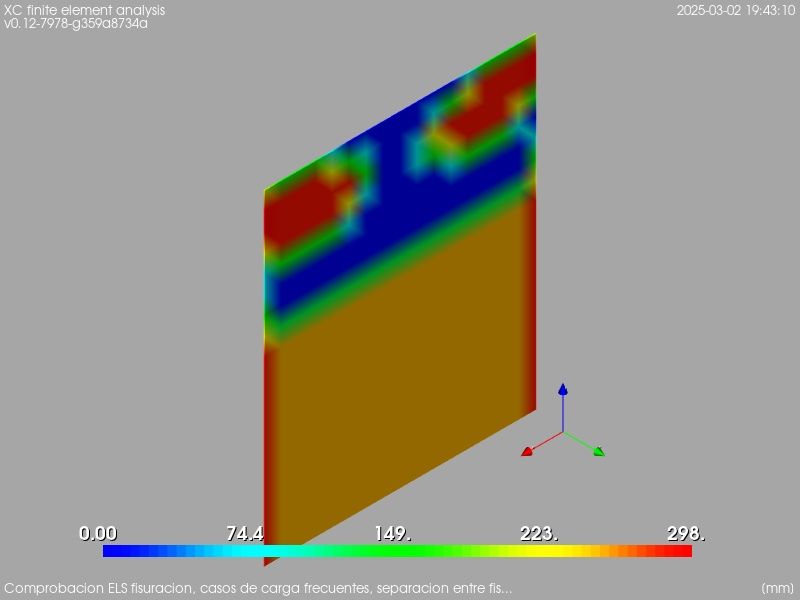
\includegraphics[width=\linewidth]{results/graphics/crackingSLS_freq/walls_rmaxSect1}
\caption{Comprobación ELS fisuración, casos de carga frecuentes. Wall, separación entre fisuras, dir. 1}
\label{SLS_frequentLoadsCrackControlwalls_rmaxSect1}
\end{center}
\end{figure}
\begin{figure}[ht]
\begin{center}
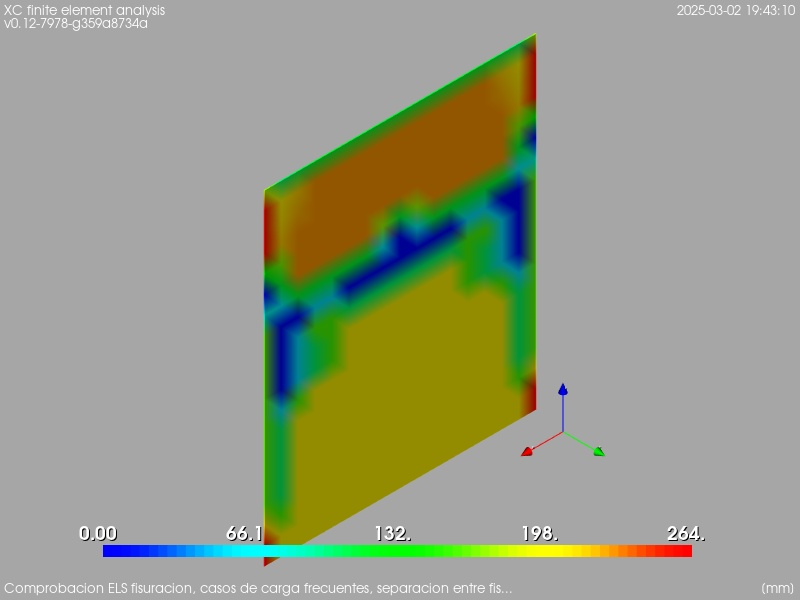
\includegraphics[width=\linewidth]{results/graphics/crackingSLS_freq/walls_rmaxSect2}
\caption{Comprobación ELS fisuración, casos de carga frecuentes. Wall, separación entre fisuras, dir. 2}
\label{SLS_frequentLoadsCrackControlwalls_rmaxSect2}
\end{center}
\end{figure}
\begin{figure}[ht]
\begin{center}
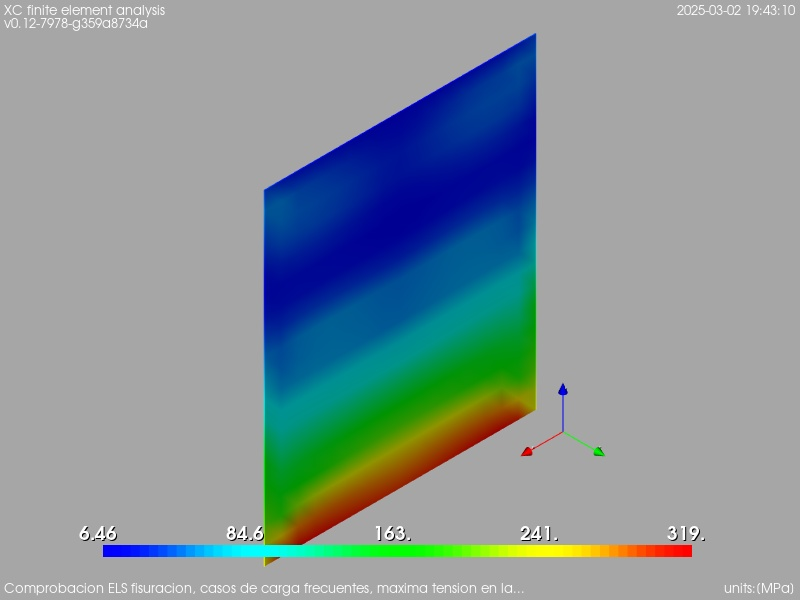
\includegraphics[width=\linewidth]{results/graphics/crackingSLS_freq/wallsigma_sSect1}
\caption{Comprobación ELS fisuración, casos de carga frecuentes. Wall, máxima tensión en la armadura, dir. 1}
\label{SLS_frequentLoadsCrackControlwallsigma_sSect1}
\end{center}
\end{figure}
\begin{figure}[ht]
\begin{center}
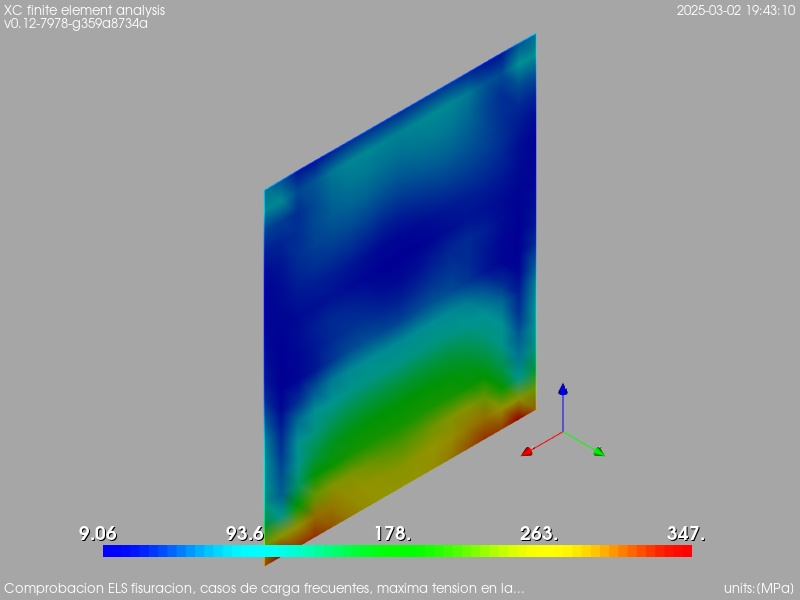
\includegraphics[width=\linewidth]{results/graphics/crackingSLS_freq/wallsigma_sSect2}
\caption{Comprobación ELS fisuración, casos de carga frecuentes. Wall, máxima tensión en la armadura, dir. 2}
\label{SLS_frequentLoadsCrackControlwallsigma_sSect2}
\end{center}
\end{figure}
\begin{figure}[ht]
\begin{center}
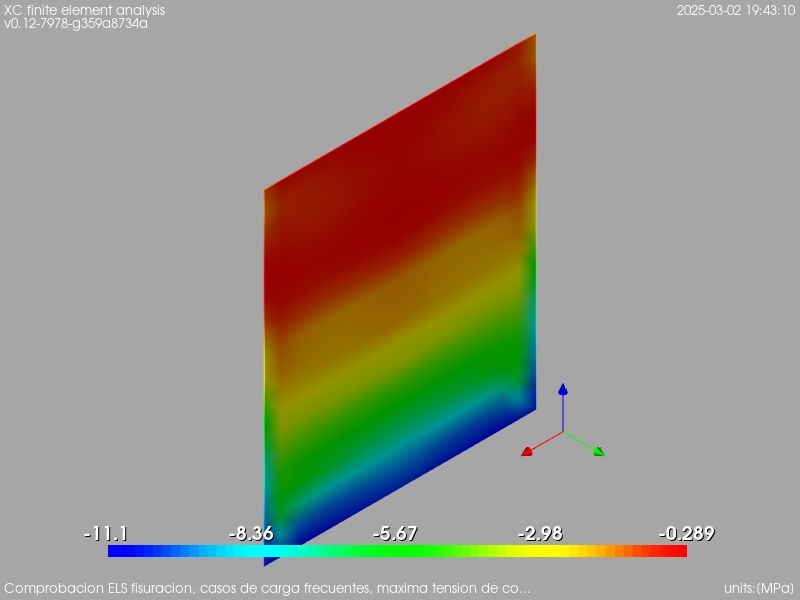
\includegraphics[width=\linewidth]{results/graphics/crackingSLS_freq/wallsigma_cSect1}
\caption{Comprobación ELS fisuración, casos de carga frecuentes. Wall, máxima tensión de compresión en el hormigón, dir. 1}
\label{SLS_frequentLoadsCrackControlwallsigma_cSect1}
\end{center}
\end{figure}
\begin{figure}[ht]
\begin{center}
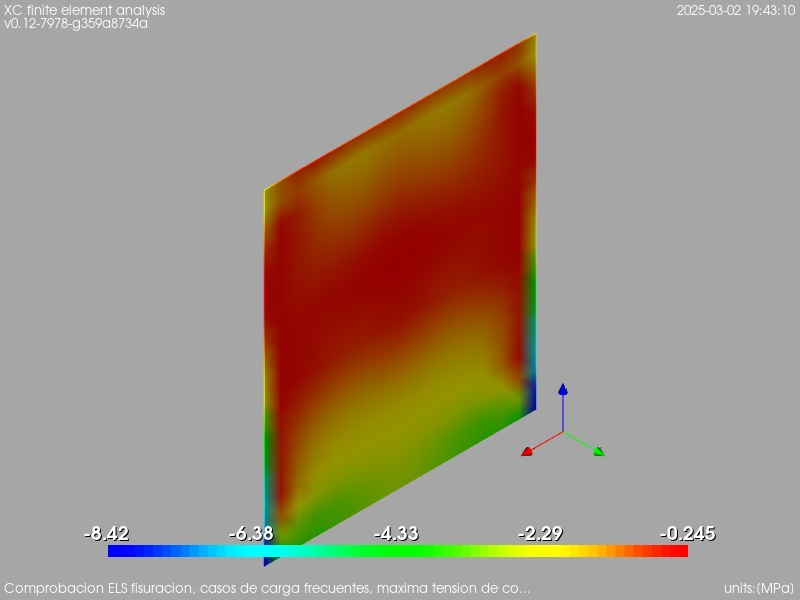
\includegraphics[width=\linewidth]{results/graphics/crackingSLS_freq/wallsigma_cSect2}
\caption{Comprobación ELS fisuración, casos de carga frecuentes. Wall, máxima tensión de compresión en el hormigón, dir. 2}
\label{SLS_frequentLoadsCrackControlwallsigma_cSect2}
\end{center}
\end{figure}
\begin{figure}[ht]
\begin{center}
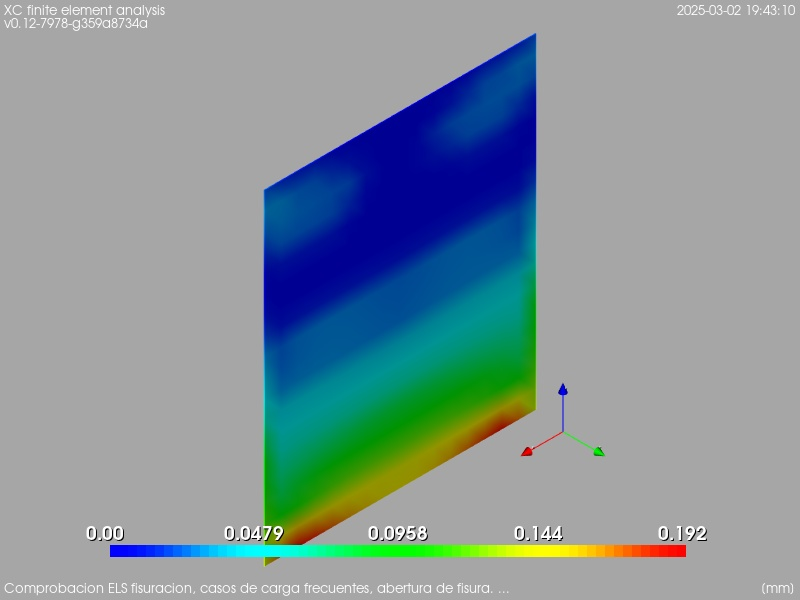
\includegraphics[width=\linewidth]{results/graphics/crackingSLS_freq/wallwkSect1}
\caption{Comprobación ELS fisuración, casos de carga frecuentes. Wall, abertura de fisura, dir. 1}
\label{SLS_frequentLoadsCrackControlwallwkSect1}
\end{center}
\end{figure}
\begin{figure}[ht]
\begin{center}
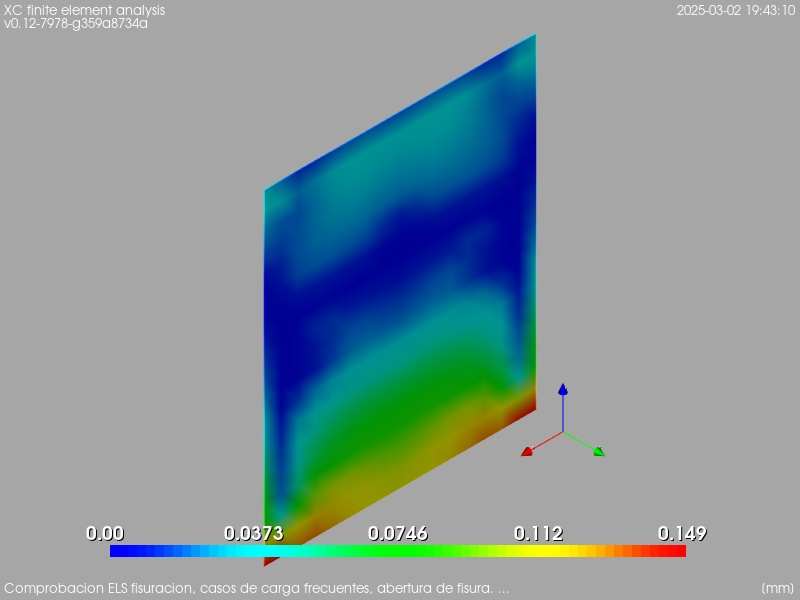
\includegraphics[width=\linewidth]{results/graphics/crackingSLS_freq/wallwkSect2}
\caption{Comprobación ELS fisuración, casos de carga frecuentes. Wall, abertura de fisura, dir. 2}
\label{SLS_frequentLoadsCrackControlwallwkSect2}
\end{center}
\end{figure}
\begin{figure}[ht]
\begin{center}
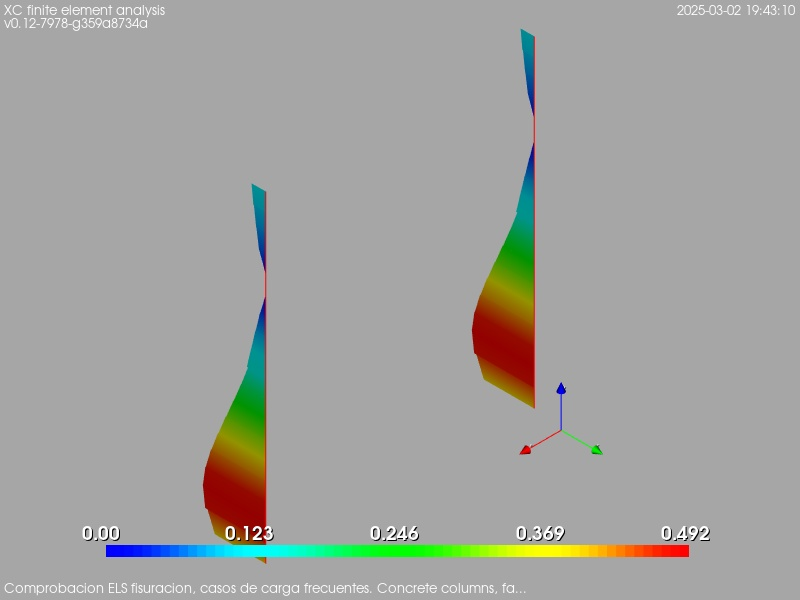
\includegraphics[width=\linewidth]{results/graphics/crackingSLS_freq/columnZconcrCF}
\caption{Comprobación ELS fisuración, casos de carga frecuentes. Concrete columns, factor de capacidad}
\label{SLS_frequentLoadsCrackControlcolumnZconcrCF}
\end{center}
\end{figure}
\begin{figure}[ht]
\begin{center}
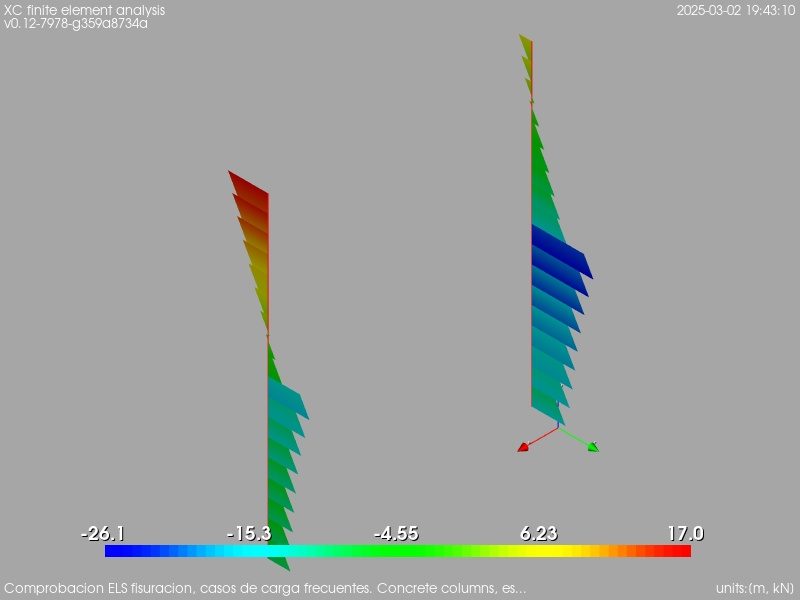
\includegraphics[width=\linewidth]{results/graphics/crackingSLS_freq/columnZconcrN}
\caption{Comprobación ELS fisuración, casos de carga frecuentes. Concrete columns, esfuerzo axil asociado al factor de capacidad}
\label{SLS_frequentLoadsCrackControlcolumnZconcrN}
\end{center}
\end{figure}
\begin{figure}[ht]
\begin{center}
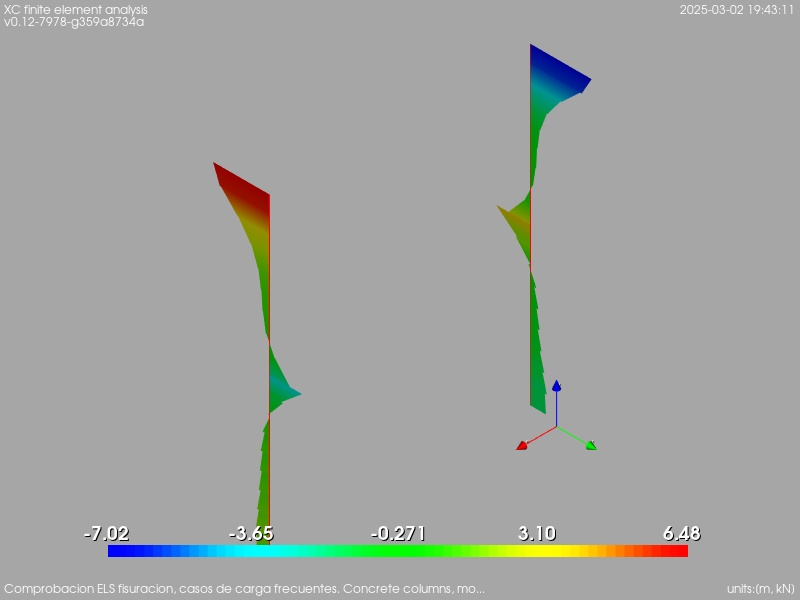
\includegraphics[width=\linewidth]{results/graphics/crackingSLS_freq/columnZconcrMy}
\caption{Comprobación ELS fisuración, casos de carga frecuentes. Concrete columns, momento flector My asociado al factor de capacidad}
\label{SLS_frequentLoadsCrackControlcolumnZconcrMy}
\end{center}
\end{figure}
\begin{figure}[ht]
\begin{center}
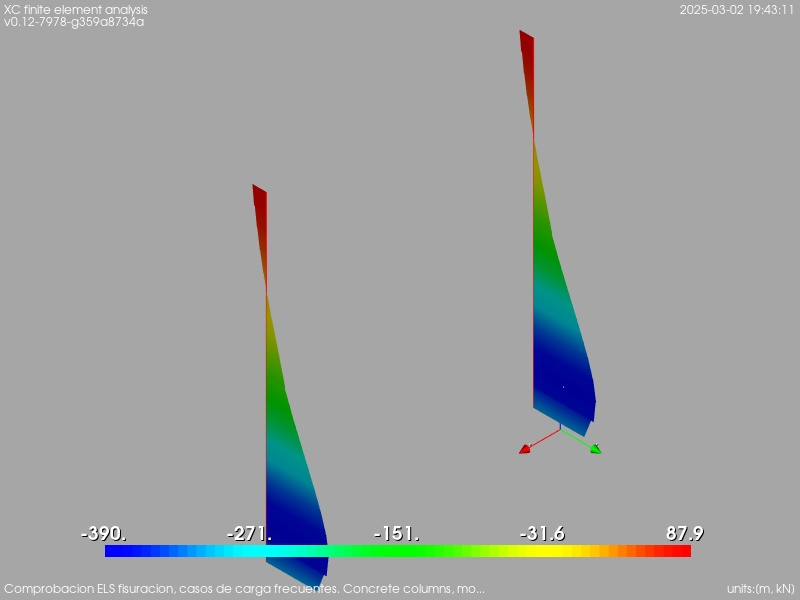
\includegraphics[width=\linewidth]{results/graphics/crackingSLS_freq/columnZconcrMz}
\caption{Comprobación ELS fisuración, casos de carga frecuentes. Concrete columns, momento flector Mz asociado al factor de capacidad}
\label{SLS_frequentLoadsCrackControlcolumnZconcrMz}
\end{center}
\end{figure}
\begin{figure}[ht]
\begin{center}
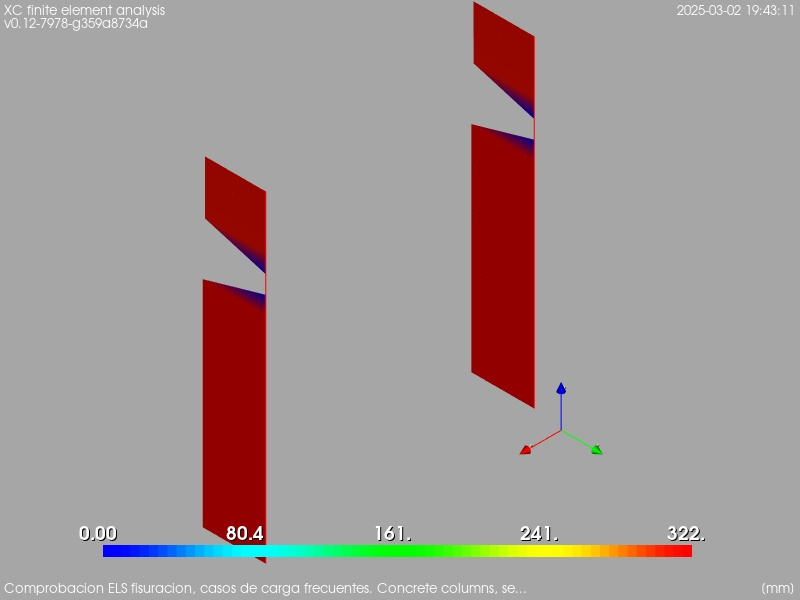
\includegraphics[width=\linewidth]{results/graphics/crackingSLS_freq/columnZconcrs_rmax}
\caption{Comprobación ELS fisuración, casos de carga frecuentes. Concrete columns, separación entre fisuras}
\label{SLS_frequentLoadsCrackControlcolumnZconcrs_rmax}
\end{center}
\end{figure}
\begin{figure}[ht]
\begin{center}
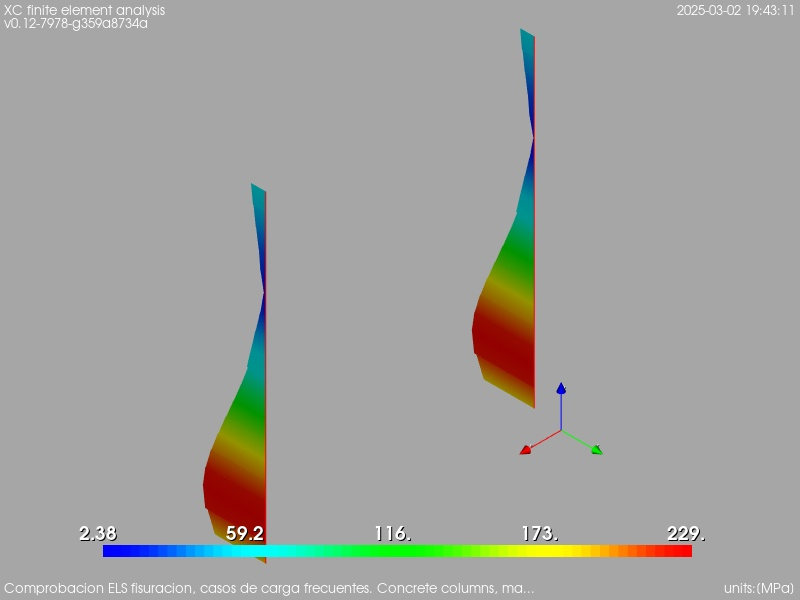
\includegraphics[width=\linewidth]{results/graphics/crackingSLS_freq/columnZconcrsigma_s}
\caption{Comprobación ELS fisuración, casos de carga frecuentes. Concrete columns, máxima tensión en la armadura}
\label{SLS_frequentLoadsCrackControlcolumnZconcrsigma_s}
\end{center}
\end{figure}
\begin{figure}[ht]
\begin{center}
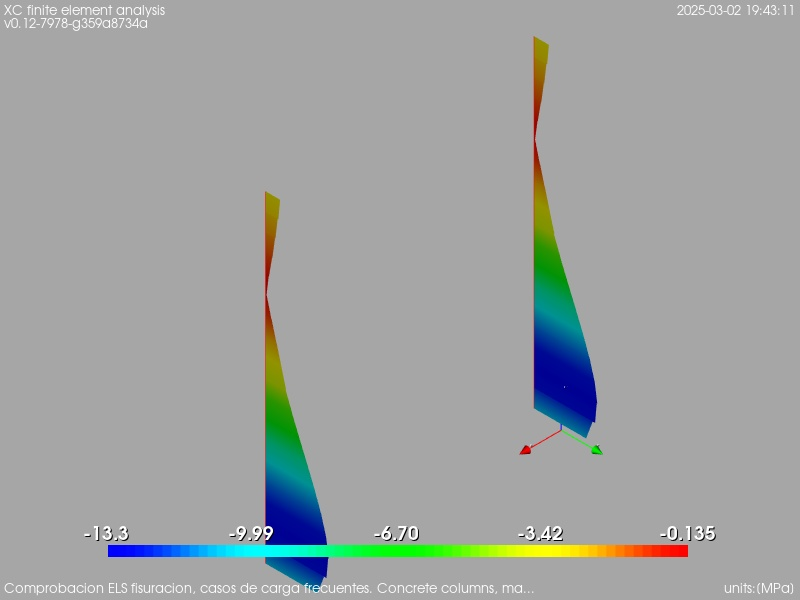
\includegraphics[width=\linewidth]{results/graphics/crackingSLS_freq/columnZconcrsigma_c}
\caption{Comprobación ELS fisuración, casos de carga frecuentes. Concrete columns, máxima tensión de compresión en el hormigón}
\label{SLS_frequentLoadsCrackControlcolumnZconcrsigma_c}
\end{center}
\end{figure}
\begin{figure}[ht]
\begin{center}
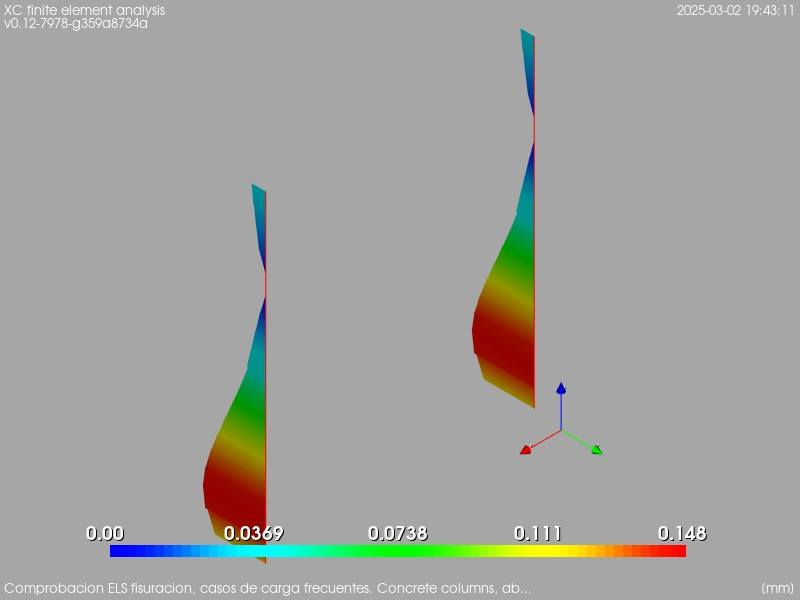
\includegraphics[width=\linewidth]{results/graphics/crackingSLS_freq/columnZconcrwk}
\caption{Comprobación ELS fisuración, casos de carga frecuentes. Concrete columns, abertura de fisura}
\label{SLS_frequentLoadsCrackControlcolumnZconcrwk}
\end{center}
\end{figure}
